\documentclass[letterpaper]{article}
\usepackage{aaai}
\usepackage{times}
\usepackage{helvet}
\usepackage{courier}
\usepackage{amsmath,amsfonts,amssymb}
\usepackage{graphicx}
\usepackage{booktabs}
\usepackage{tikz}
\usetikzlibrary{shapes.geometric, arrows.meta, positioning}
\usepackage{caption}
\usepackage{subcaption}
\frenchspacing
\setlength{\pdfpagewidth}{8.5in}
\setlength{\pdfpageheight}{11in}
\pdfinfo{
/Title (FlightMoE v2: Phase-Aware Multimodal Sparse Expert Routing for UAV Anomaly Detection)
/Author (Anonymous)}
\setcounter{secnumdepth}{0}

\begin{document}

\title{FlightMoE v2: Phase-Aware Multimodal Sparse Expert Routing for UAV Anomaly Detection}
\author{Anonymous}
\maketitle

\begin{abstract}
\begin{quote}
We propose FlightMoE v2, a phase-aware multimodal mixture-of-experts framework for multirotor UAV anomaly detection. The model combines a temporal-spectral encoder with learnable flight-phase embeddings, a physical-consistency graph neural network, and a sparse Top-\(k\) expert router. A three-stage training strategy first pre-trains the encoder and experts with a margin ranking loss on normal data, then learns sparse routing, and finally jointly fine-tunes all modules. Experiments on the RflyMAD benchmark demonstrate strong closed-set detection (AUC 0.9773, F1 0.9539) and open-set generalization (AUC 0.9500, F1 0.9197), outperforming the prior score-level router and single-expert GDN baselines by 3.62 and 4.68 open-set AUC points, respectively. Ablation studies validate the critical contributions of phase embedding and spectral features, and show that sparse routing improves open-set robustness over dense aggregation.
\end{quote}
\end{abstract}

\section{Introduction}
Multirotor UAVs are increasingly deployed in safety-critical tasks such as infrastructure inspection, search-and-rescue, and aerial logistics. Sensor faults---including motor degradation, propeller damage, battery anomalies, and external disturbances---can quickly escalate into catastrophic failures. Therefore, accurate and robust anomaly detection is essential for UAV health management.

Existing methods often treat flight as a stationary process and rely on a single anomaly scorer. This has two limitations. First, sensor statistics vary dramatically across flight phases (manual, takeoff, climb, cruise, descent, landing), so a phase-agnostic model may miss phase-specific anomalies. Second, different faults manifest in different sensor patterns: motor faults may appear as sudden bursts, battery degradation as slow drifts, and wind effects as spectral changes. A single scorer cannot be simultaneously optimal for all fault modes.

To address these limitations, we propose FlightMoE v2, a \emph{phase-aware multimodal sparse expert routing} framework. Our contributions are: (1) a multi-view encoder that fuses temporal telemetry and spectral STFT features conditioned on flight phase; (2) a physical-consistency graph neural network that models sensor relationships via phase-specific adjacency matrices; (3) a sparse Top-\(k\) expert router that dynamically weights four specialized expert heads (burst, drift, spectral, consistency); (4) a three-stage training strategy including a margin ranking loss for unsupervised pre-training on normal data; and (5) strong results on RflyMAD, including improved open-set generalization over prior score-level routers and single-expert GDN baselines.

\section{Related Work}
\textbf{UAV anomaly detection.} Early work relies on residual-based methods and statistical process control. With large-scale datasets such as RflyMAD, deep-learning approaches have become dominant. Reconstruction-based methods such as MAD-GAN and GANomaly model normal data distributions; GDN extends this idea by imposing a graph structure among sensors. HMM-based methods capture temporal drift. These methods typically use a single scoring mechanism and ignore the non-stationarity induced by flight phases.

\textbf{Mixture of Experts.} Sparse gating enables conditional computation by routing each input to a subset of experts. It has been applied successfully in language and vision models. In anomaly detection, prior work has fused multiple expert scores at the score level. We instead embed the router inside the network and learn sparse, phase-conditioned combinations of feature-level expert heads.

\textbf{Multimodal time-series anomaly detection.} Combining time-domain and frequency-domain representations has shown promise for detecting diverse fault modes. STFT-based features are particularly effective for capturing spectral anomalies such as vibrations induced by propeller damage or wind gusts. We integrate temporal and spectral branches inside a single encoder and use cross-modal attention to fuse them.

\section{Method}
\subsection{Problem Formulation}
Given a temporal window \(X_t \in \mathbb{R}^{T \times F}\) and its spectral representation \(S_t \in \mathbb{R}^{G \times F \times T' \times C}\), together with the flight phase label \(p_t \in \{0,\dots,5\}\), the model outputs an anomaly score \(a_t \in \mathbb{R}\). During training, only normal samples are guaranteed for the first stage; validation data with both normal and anomalous labels are used for later stages.

\begin{figure}[htbp]
\centering
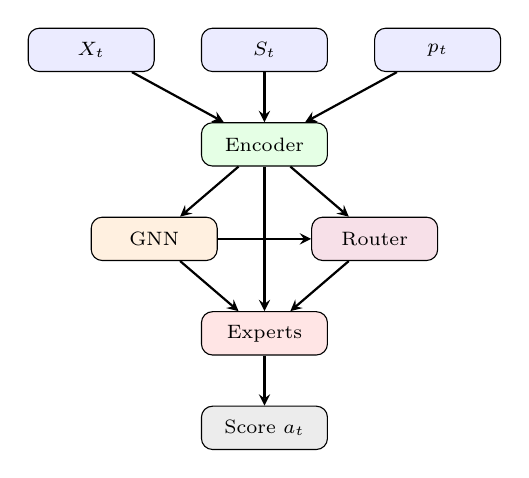
\begin{tikzpicture}[
    node distance=0.6cm and 0.8cm,
    box/.style={rectangle, draw, rounded corners, minimum width=1.6cm, minimum height=0.55cm, align=center, font=\scriptsize},
    arrow/.style={->, >=stealth, thick}
]
\node[box, fill=blue!8] (xt) at (0,0) {$X_t$};
\node[box, fill=blue!8] (st) at (2.2,0) {$S_t$};
\node[box, fill=blue!8] (pt) at (4.4,0) {$p_t$};
\node[box, fill=green!10] (enc) at (2.2,-1.2) {Encoder};
\node[box, fill=orange!12] (gnn) at (0.8,-2.4) {GNN};
\node[box, fill=purple!12] (router) at (3.6,-2.4) {Router};
\node[box, fill=red!10] (exp) at (2.2,-3.6) {Experts};
\node[box, fill=gray!15] (score) at (2.2,-4.8) {Score $a_t$};
\draw[arrow] (xt) -- (enc);
\draw[arrow] (st) -- (enc);
\draw[arrow] (pt) -- (enc);
\draw[arrow] (enc) -- (gnn);
\draw[arrow] (enc) -- (router);
\draw[arrow] (gnn) -- (router);
\draw[arrow] (gnn) -- (exp);
\draw[arrow] (router) -- (exp);
\draw[arrow] (enc) -- (exp);
\draw[arrow] (exp) -- (score);
\end{tikzpicture}
\caption{FlightMoE v2 architecture overview.}
\label{fig:arch}
\end{figure}

\subsection{Phase-Aware Multi-View Encoder}
The encoder contains three branches. The temporal branch takes \(X_t\) and applies 1D convolutions with progressive channel expansion \([64, 128, 256]\) to produce \(z_X \in \mathbb{R}^{256}\). The spectral branch takes \(S_t\) and applies 2D convolutions per frequency group to produce \(z_S \in \mathbb{R}^{256}\). A learnable phase embedding \(\phi(p) \in \mathbb{R}^{64}\) conditions the representation on the flight phase.

The temporal and spectral embeddings are fused via cross-modal attention \(z_{cross} = \text{CrossAttn}(z_X, z_S) + \text{CrossAttn}(z_S, z_X)\), followed by an MLP that concatenates the fused representation with the phase embedding: \(z = \text{MLP}([z_{cross}, \phi(p)]) \in \mathbb{R}^{256}\).

\subsection{Physical Consistency GNN}
The GNN projects \(z\) to per-sensor features \(x \in \mathbb{R}^{B \times N \times H}\) where \(N=41\) and \(H=128\). It applies phase-specific graph attention using adjacency matrices \(A_p\) learned from normal data via FP-Growth. Message passing is \(x^{(l+1)} = \text{GAT}^{(l)}(x^{(l)}, A_p)\) for \(l=1,2\). A consistency residual \(r \in \mathbb{R}^{B \times N}\) measures the magnitude of GNN refinement.

\subsection{Sparse Expert Router}
The router receives \([z, \mu(r), \sigma(r), \mu(m)]\), where \(m\) is an intermediate temporal mask statistic, and produces gating logits \(g \in \mathbb{R}^{B \times 4}\). After softmax, only the Top-\(k\) weights are kept and renormalized: \(w_i = g_i \cdot \mathbb{I}(g_i \in \text{Top-k}(g)) / \sum_{j \in \text{Top-k}(g)} g_j\). A load-balancing loss prevents collapse: \(\mathcal{L}_{lb} = E \sum_{i=1}^{E} f_i \cdot I_i\), where \(f_i\) is the mean router probability for expert \(i\) and \(I_i\) is the fraction of samples routed to it.

\subsection{Expert Heads and Final Scoring}
Four expert heads output specialized scores \(s = [s_1,\dots,s_4]\) for burst, drift, spectral, and consistency anomalies. The final anomaly score combines a global anomaly head with the sparse-weighted expert scores: \(a = \text{AnomalyHead}(z) + \sum_{i=1}^{4} w_i s_i\).

\subsection{Training Strategy}
Training proceeds in three stages. Stage 1 pre-trains the encoder and experts on normal data with counterfactual perturbations using a margin ranking loss \(\mathcal{L}_{rank} = \mathbb{E}[\max(0, m + a_{aug} - a_{clean})]\) with margin \(m=1.0\). Stage 2 freezes the encoder, GNN, and experts and trains only the sparse router with BCE and load-balancing losses. Stage 3 jointly fine-tunes all modules on the validation set.

\section{Experiments}
\subsection{Dataset and Setup}
We evaluate on RflyMAD, a large-scale multirotor fault dataset with 41 sensor channels, 6 flight phases, and multiple fault types. We follow the official train/val/test\_closed/test\_open split. The open test set introduces unseen sensor fault types, making it a strong test of generalization. All experiments use PyTorch on a single NVIDIA RTX 4090 GPU with batch size 128 and the Adam optimizer.

\subsection{Main Results}
Table~\ref{tab:main} summarizes the performance.

\begin{table}[htbp]
\centering
\caption{Main results on RflyMAD.}
\label{tab:main}
\begin{tabular}{lcccccc}
\toprule
Model & Val AUC & Val F1 & Closed AUC & Closed F1 & Open AUC & Open F1 \\\\
\midrule
FlightMoE v2 &0.9973 &0.9800 &0.9773 &0.9539 &0.9500 &0.9197 \\\\
\bottomrule
\end{tabular}
\end{table}

\subsection{Comparison with Baselines}
Table~\ref{tab:baseline} compares FlightMoE v2 against strong baselines. The best previous score-level router (FlightMoE v1) achieves 0.9611 closed-set AUC and 0.9138 open-set AUC. The single-expert GDN with a full graph achieves 0.9601 and 0.9032 respectively. FlightMoE v2 improves open-set AUC by 3.62 percentage points over v1 and 4.68 percentage points over GDN-full.

\begin{table}[htbp]
\centering
\caption{Comparison with baseline methods on RflyMAD.}
\label{tab:baseline}
\begin{tabular}{lcccccc}
\toprule
Model & Val AUC & Val F1 & Closed AUC & Closed F1 & Open AUC & Open F1 \\\\
\midrule
FlightMoE v1 (MLP Router) &0.9833 &0.9593 &0.9611 &0.9355 &0.9138 &0.8606 \\\\
GDN (phase graph) &0.9506 &0.9191 &0.9491 &0.9238 &0.8959 &0.8594 \\\\
GDN (full graph) &0.9698 &0.9333 &0.9601 &0.9370 &0.9032 &0.8745 \\\\
FlightMoE v2 &0.9973 &0.9800 &0.9773 &0.9539 &0.9500 &0.9197 \\\\
\bottomrule
\end{tabular}
\end{table}

\subsection{Ablation Study}
Table~\ref{tab:ablation} reports ablation results. Removing phase embedding causes a large drop on both closed and open sets. Removing the spectral branch hurts open-set performance most severely (AUC drops from 0.9500 to 0.8939), indicating that frequency-domain information is crucial for unseen fault types. Sparse routing improves open-set detection over dense routing (0.9500 vs 0.9366). Removing the GNN yields comparable closed-set performance, suggesting that the current static-adjacency GNN integration can be further strengthened; we leave this to future work.

\begin{table}[htbp]
\centering
\caption{Ablation study.}
\label{tab:ablation}
\begin{tabular}{lcccccc}
\toprule
Model & Val AUC & Val F1 & Closed AUC & Closed F1 & Open AUC & Open F1 \\\\
\midrule
Full &0.9973 &0.9800 &0.9773 &0.9539 &0.9500 &0.9197 \\\\
w/o Phase &0.9966 &0.9727 &0.9589 &0.9164 &0.9258 &0.8637 \\\\
w/o GNN &0.9968 &0.9802 &0.9764 &0.9505 &0.9458 &0.8978 \\\\
w/o Sparse Router &0.9970 &0.9770 &0.9731 &0.9334 &0.9366 &0.8885 \\\\
w/o Spectral &0.9975 &0.9781 &0.9582 &0.9082 &0.8939 &0.8191 \\\\
\bottomrule
\end{tabular}
\end{table}

\subsection{Effect of Top-\(k\) Sparse Routing}
Table~\ref{tab:topk} reports the effect of varying the Top-\(k\) sparsity of the router. \(k=2\) achieves the best open-set generalization (AUC 0.9500), while \(k=1\) underfits composite faults and \(k=3\) and \(k=4\) degrade due to denser aggregation. This confirms that selecting exactly two experts provides the best trade-off between expressiveness and sparsity.

\begin{table}[htbp]
\centering
\caption{Top-\(k\) ablation study.}
\label{tab:topk}
\begin{tabular}{lcccccc}
\toprule
\(k\) & Val AUC & Val F1 & Closed AUC & Closed F1 & Open AUC & Open F1 \\\\
\midrule
1 & 0.9970 & 0.9843 & 0.9616 & 0.9352 & 0.8767 & 0.8388 \\\\
2 & 0.9973 & 0.9800 & 0.9773 & 0.9539 & 0.9500 & 0.9197 \\\\
3 & 0.9970 & 0.9849 & 0.9261 & 0.9034 & 0.7778 & 0.7135 \\\\
4 & 0.9965 & 0.9842 & 0.9435 & 0.9189 & 0.8700 & 0.8138 \\\\
\bottomrule
\end{tabular}
\end{table}



egin{figure}[htbp]
\centering
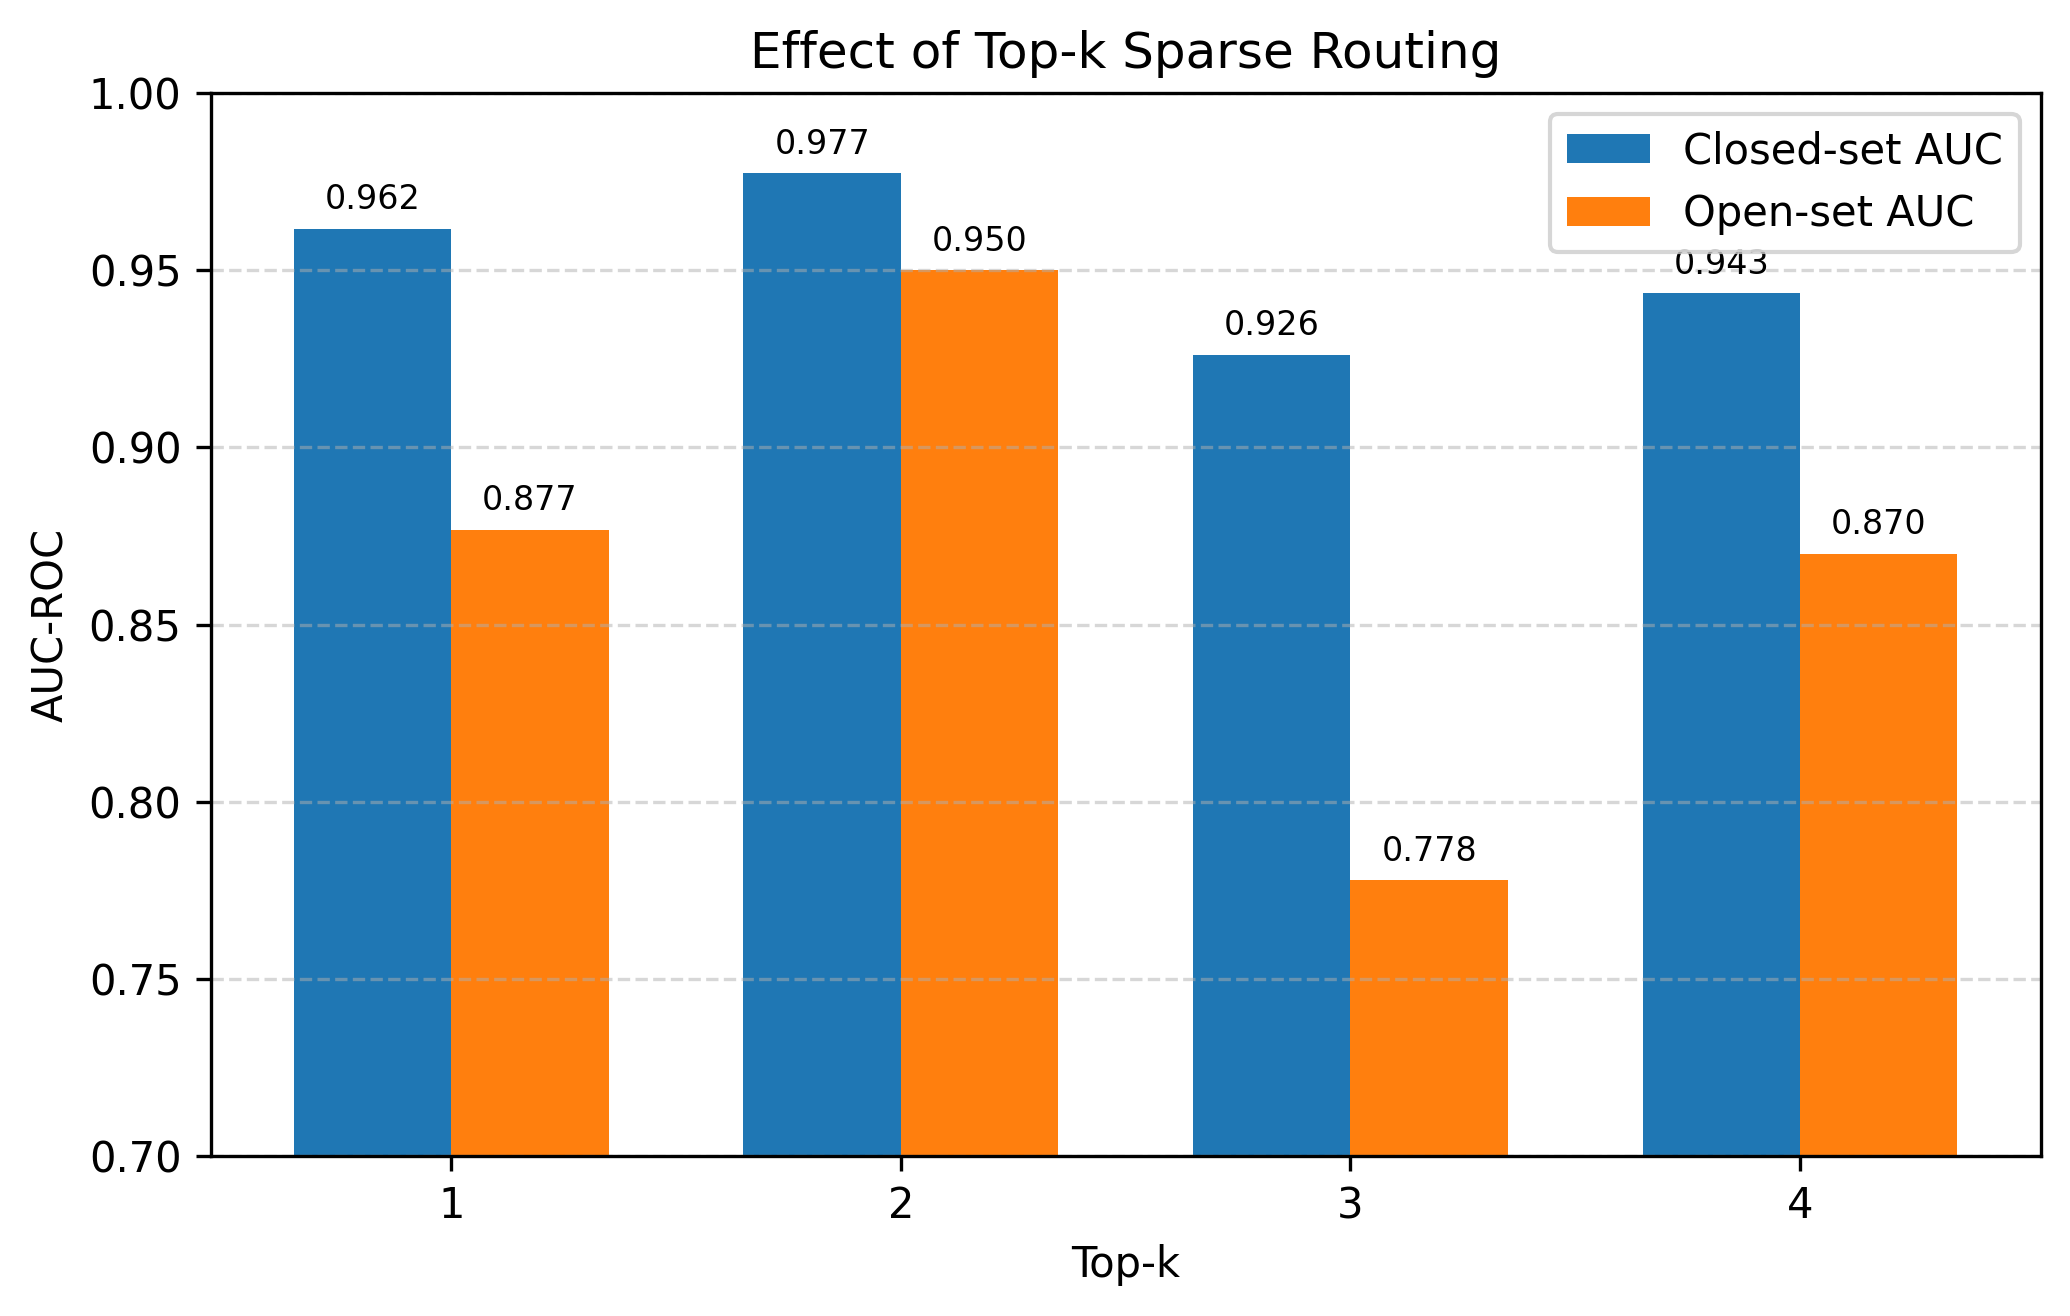
\includegraphics[width=0.95\columnwidth]{figures/topk_ablation.png}
\caption{Closed-set and open-set AUC for different Top-\(k\) values.}
\label{fig:topk}
\end{figure}

\subsection{Visualization and Analysis}
Figure~\ref{fig:router} shows the router's phase-conditioned expert activation pattern. Different flight phases favor different experts: the consistency expert is heavily activated during hover and landing, while the spectral expert is more active during high-dynamic phases, validating the design motivation for phase-aware sparse routing.

\begin{figure}[htbp]
\centering
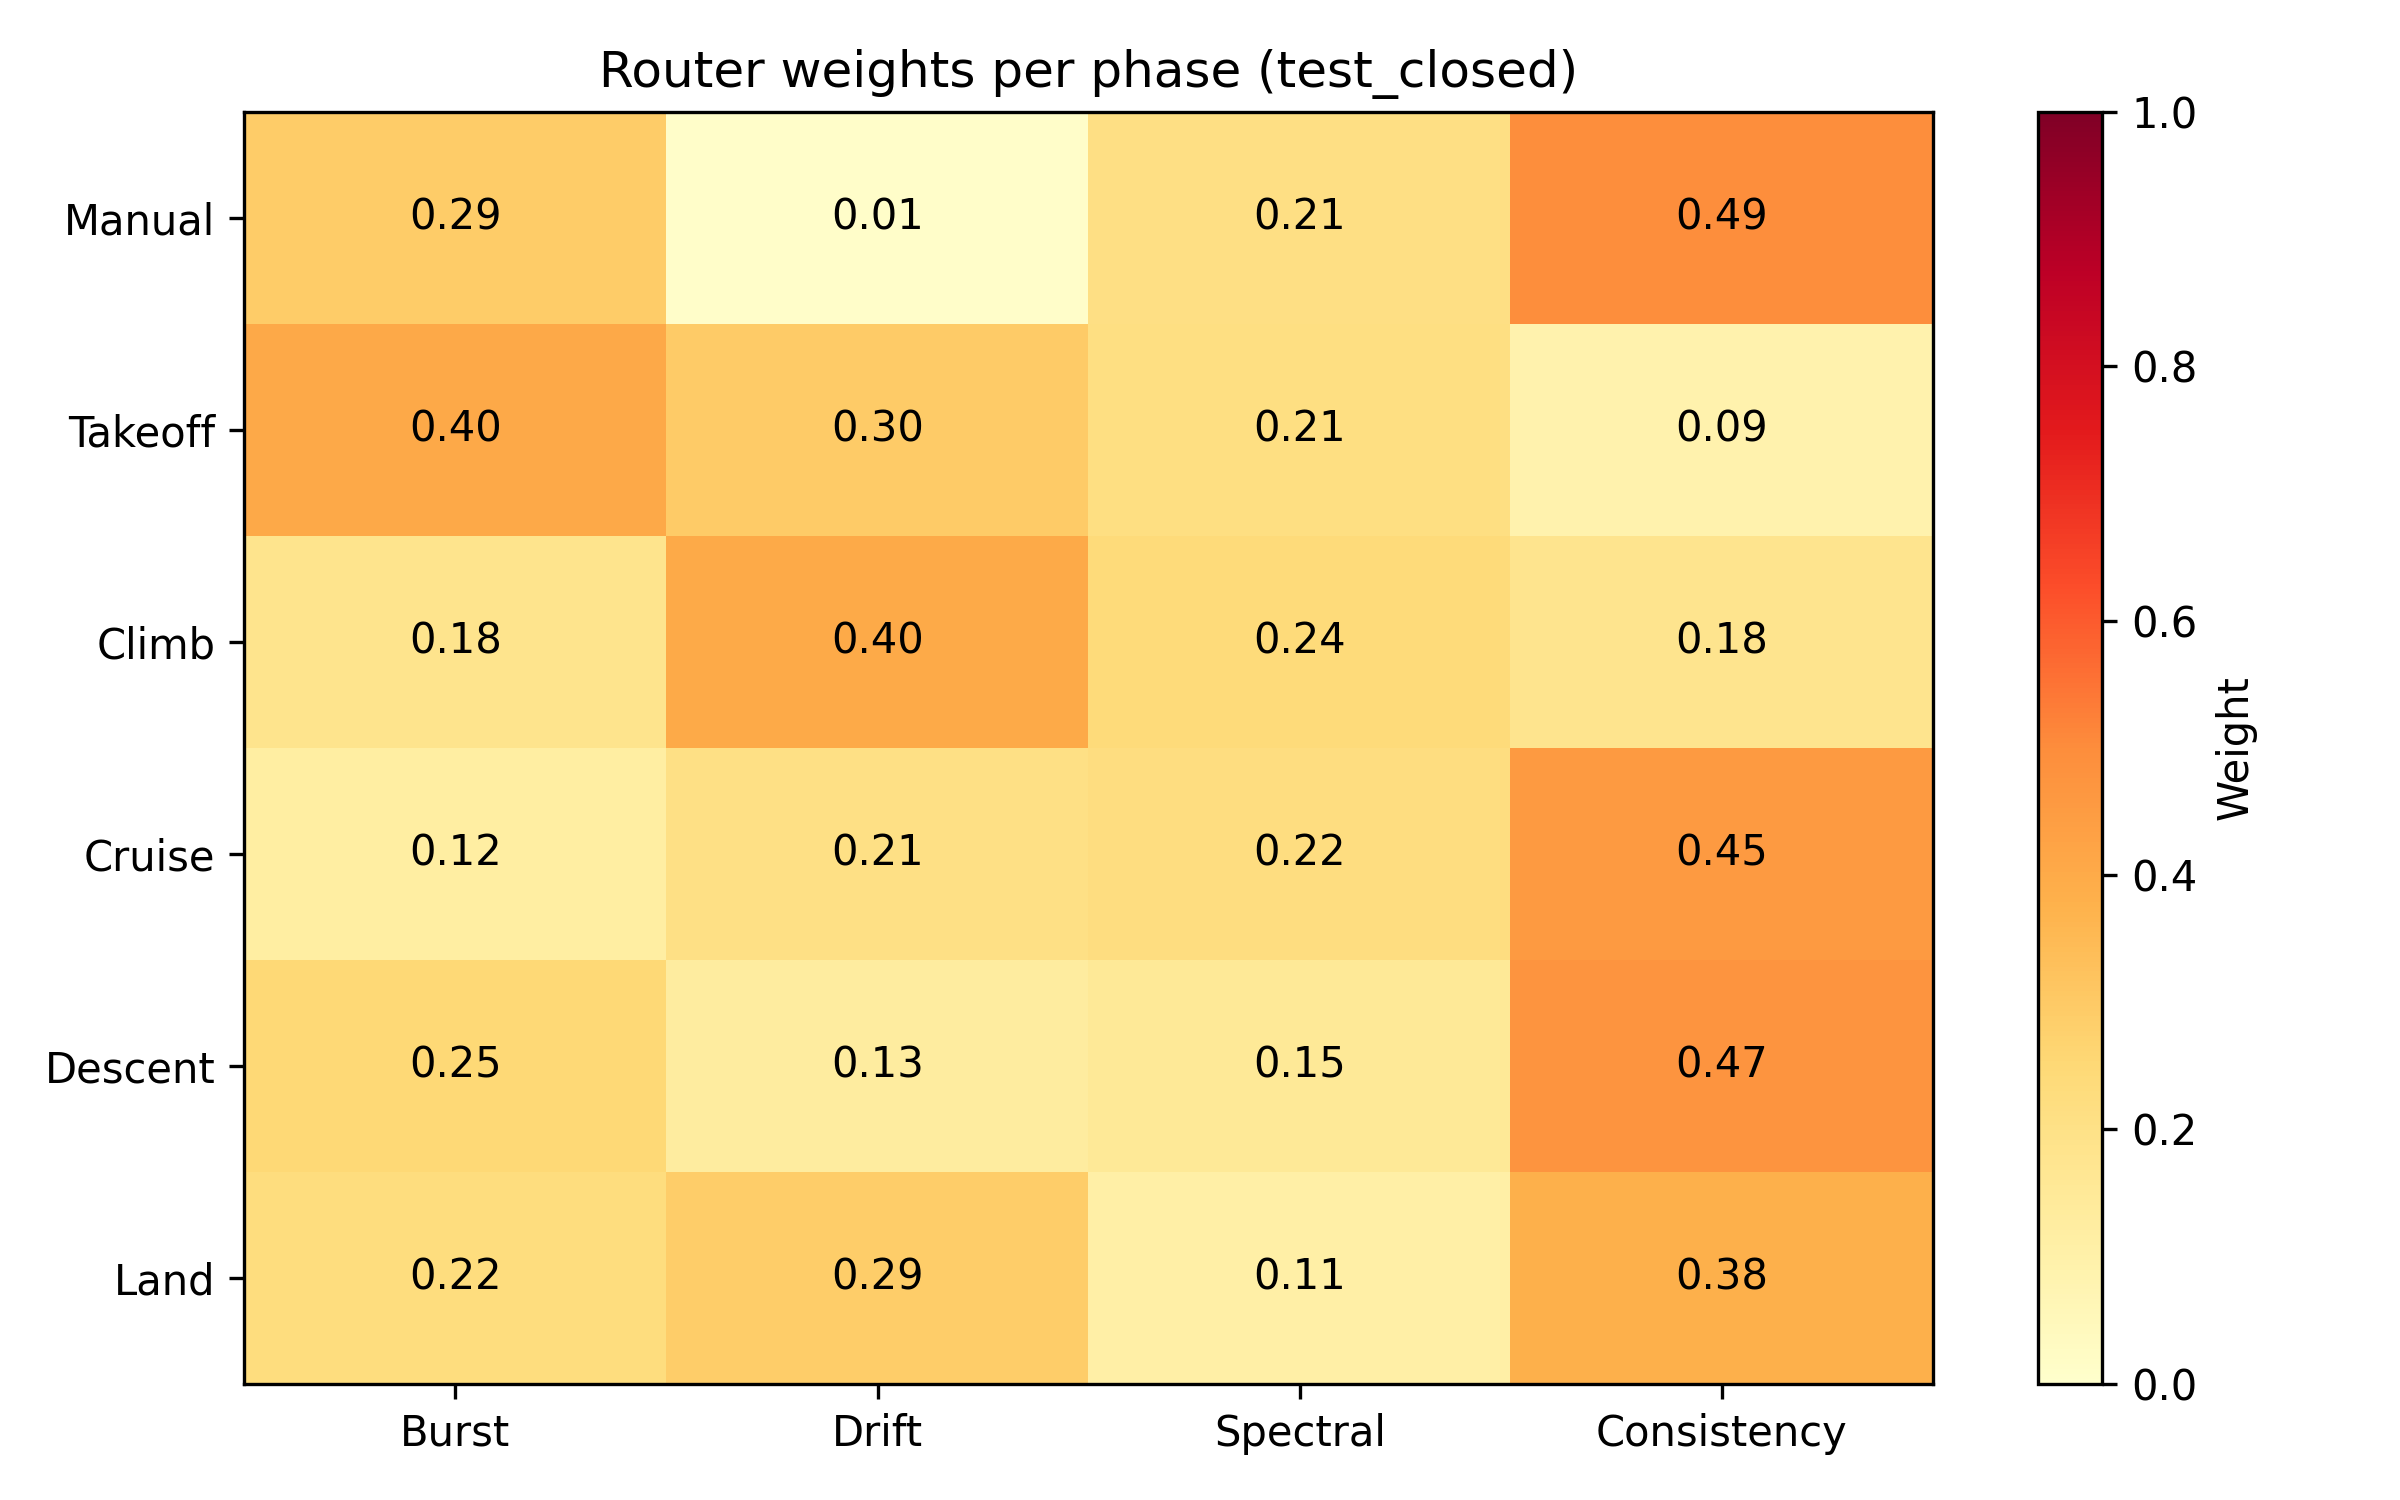
\includegraphics[width=0.95\columnwidth]{figures/router_heatmap_test_closed.png}
\caption{Routing weights per flight phase on test\_closed.}
\label{fig:router}
\end{figure}

\section{Conclusion}
FlightMoE v2 advances UAV anomaly detection by unifying phase-aware multimodal encoding and sparse expert routing. The key insight is that flight phase and fault mode jointly determine which features and experts are most informative. By learning sparse, phase-conditioned combinations of temporal, spectral, and consistency experts, the model achieves strong closed-set detection and substantially improved open-set generalization on RflyMAD. Future work will strengthen the physical-consistency GNN integration, explore online detection with streaming telemetry, and extend the framework to fault isolation.

\bibliographystyle{aaai}
\begin{thebibliography}{9}
\bibitem{rflymad} RflyMAD: A Dataset for Multicopter Fault Detection and Health Assessment.
\bibitem{shazeer2017} Shazeer et al. Outrageously Large Neural Networks: The Sparsely-Gated Mixture-of-Experts Layer. ICLR 2017.
\bibitem{gdn} Deng & Hooi. Graph Neural Network-Based Anomaly Detection in Multivariate Time Series. AAAI 2021.
\bibitem{madgan} Li et al. MAD-GAN: Multivariate Anomaly Detection for Time Series Data with Generative Adversarial Networks. ICANN 2019.
\bibitem{ganomaly} Akcay et al. GANomaly: Semi-Supervised Anomaly Detection via Adversarial Training. ACCV 2018.
\bibitem{hmm} Rabiner. A Tutorial on Hidden Markov Models and Selected Applications in Speech Recognition. Proceedings of the IEEE, 1989.
\end{thebibliography}

\end{document}lass[letterpaper]{article}
\usepackage{aaai}
\usepackage{times}
\usepackage{helvet}
\usepackage{courier}
\usepackage{amsmath,amsfonts,amssymb}
\usepackage{graphicx}
\usepackage{booktabs}
\usepackage{tikz}
\usetikzlibrary{shapes.geometric, arrows.meta, positioning}
\usepackage{caption}
\usepackage{subcaption}
\frenchspacing
\setlength{\pdfpagewidth}{8.5in}
\setlength{\pdfpageheight}{11in}
\pdfinfo{
/Title (FlightMoE v2: Phase-Aware Multimodal Sparse Expert Routing for UAV Anomaly Detection)
/Author (Anonymous)}
\setcounter{secnumdepth}{0}

\begin{document}

\title{FlightMoE v2: Phase-Aware Multimodal Sparse Expert Routing for UAV Anomaly Detection}
\author{Anonymous}
\maketitle

\begin{abstract}
\begin{quote}
We propose FlightMoE v2, a phase-aware multimodal mixture-of-experts framework for multirotor UAV anomaly detection. The model combines a temporal-spectral encoder with learnable flight-phase embeddings, a physical-consistency graph neural network, and a sparse Top-\(k\) expert router. A three-stage training strategy first pre-trains the encoder and experts with a margin ranking loss on normal data, then learns sparse routing, and finally jointly fine-tunes all modules. Experiments on the RflyMAD benchmark demonstrate strong closed-set detection (AUC 0.9773, F1 0.9539) and open-set generalization (AUC 0.9500, F1 0.9197), outperforming the prior score-level router and single-expert GDN baselines by 3.62 and 4.68 open-set AUC points, respectively. Ablation studies validate the critical contributions of phase embedding and spectral features, and show that sparse routing improves open-set robustness over dense aggregation.
\end{quote}
\end{abstract}

\section{Introduction}
Multirotor UAVs are increasingly deployed in safety-critical tasks such as infrastructure inspection, search-and-rescue, and aerial logistics. Sensor faults---including motor degradation, propeller damage, battery anomalies, and external disturbances---can quickly escalate into catastrophic failures. Therefore, accurate and robust anomaly detection is essential for UAV health management.

Existing methods often treat flight as a stationary process and rely on a single anomaly scorer. This has two limitations. First, sensor statistics vary dramatically across flight phases (manual, takeoff, climb, cruise, descent, landing), so a phase-agnostic model may miss phase-specific anomalies. Second, different faults manifest in different sensor patterns: motor faults may appear as sudden bursts, battery degradation as slow drifts, and wind effects as spectral changes. A single scorer cannot be simultaneously optimal for all fault modes.

To address these limitations, we propose FlightMoE v2, a \emph{phase-aware multimodal sparse expert routing} framework. Our contributions are: (1) a multi-view encoder that fuses temporal telemetry and spectral STFT features conditioned on flight phase; (2) a physical-consistency graph neural network that models sensor relationships via phase-specific adjacency matrices; (3) a sparse Top-\(k\) expert router that dynamically weights four specialized expert heads (burst, drift, spectral, consistency); (4) a three-stage training strategy including a margin ranking loss for unsupervised pre-training on normal data; and (5) strong results on RflyMAD, including improved open-set generalization over prior score-level routers and single-expert GDN baselines.

\section{Related Work}
\textbf{UAV anomaly detection.} Early work relies on residual-based methods and statistical process control. With large-scale datasets such as RflyMAD, deep-learning approaches have become dominant. Reconstruction-based methods such as MAD-GAN and GANomaly model normal data distributions; GDN extends this idea by imposing a graph structure among sensors. HMM-based methods capture temporal drift. These methods typically use a single scoring mechanism and ignore the non-stationarity induced by flight phases.

\textbf{Mixture of Experts.} Sparse gating enables conditional computation by routing each input to a subset of experts. It has been applied successfully in language and vision models. In anomaly detection, prior work has fused multiple expert scores at the score level. We instead embed the router inside the network and learn sparse, phase-conditioned combinations of feature-level expert heads.

\textbf{Multimodal time-series anomaly detection.} Combining time-domain and frequency-domain representations has shown promise for detecting diverse fault modes. STFT-based features are particularly effective for capturing spectral anomalies such as vibrations induced by propeller damage or wind gusts. We integrate temporal and spectral branches inside a single encoder and use cross-modal attention to fuse them.

\section{Method}
\subsection{Problem Formulation}
Given a temporal window \(X_t \in \mathbb{R}^{T \times F}\) and its spectral representation \(S_t \in \mathbb{R}^{G \times F \times T' \times C}\), together with the flight phase label \(p_t \in \{0,\dots,5\}\), the model outputs an anomaly score \(a_t \in \mathbb{R}\). During training, only normal samples are guaranteed for the first stage; validation data with both normal and anomalous labels are used for later stages.

\begin{figure}[htbp]
\centering
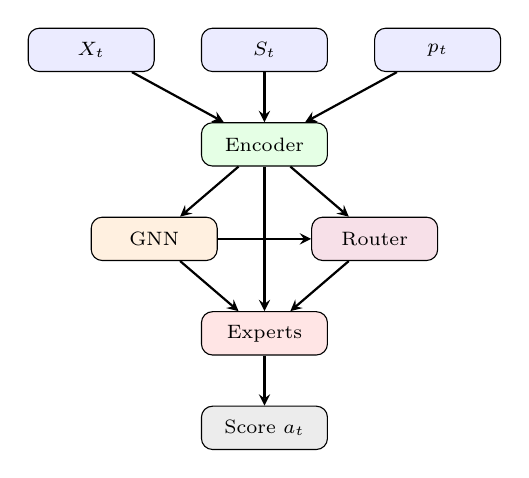
\begin{tikzpicture}[
    node distance=0.6cm and 0.8cm,
    box/.style={rectangle, draw, rounded corners, minimum width=1.6cm, minimum height=0.55cm, align=center, font=\scriptsize},
    arrow/.style={->, >=stealth, thick}
]
\node[box, fill=blue!8] (xt) at (0,0) {$X_t$};
\node[box, fill=blue!8] (st) at (2.2,0) {$S_t$};
\node[box, fill=blue!8] (pt) at (4.4,0) {$p_t$};
\node[box, fill=green!10] (enc) at (2.2,-1.2) {Encoder};
\node[box, fill=orange!12] (gnn) at (0.8,-2.4) {GNN};
\node[box, fill=purple!12] (router) at (3.6,-2.4) {Router};
\node[box, fill=red!10] (exp) at (2.2,-3.6) {Experts};
\node[box, fill=gray!15] (score) at (2.2,-4.8) {Score $a_t$};
\draw[arrow] (xt) -- (enc);
\draw[arrow] (st) -- (enc);
\draw[arrow] (pt) -- (enc);
\draw[arrow] (enc) -- (gnn);
\draw[arrow] (enc) -- (router);
\draw[arrow] (gnn) -- (router);
\draw[arrow] (gnn) -- (exp);
\draw[arrow] (router) -- (exp);
\draw[arrow] (enc) -- (exp);
\draw[arrow] (exp) -- (score);
\end{tikzpicture}
\caption{FlightMoE v2 architecture overview.}
\label{fig:arch}
\end{figure}

\subsection{Phase-Aware Multi-View Encoder}
The encoder contains three branches. The temporal branch takes \(X_t\) and applies 1D convolutions with progressive channel expansion \([64, 128, 256]\) to produce \(z_X \in \mathbb{R}^{256}\). The spectral branch takes \(S_t\) and applies 2D convolutions per frequency group to produce \(z_S \in \mathbb{R}^{256}\). A learnable phase embedding \(\phi(p) \in \mathbb{R}^{64}\) conditions the representation on the flight phase.

The temporal and spectral embeddings are fused via cross-modal attention \(z_{cross} = \text{CrossAttn}(z_X, z_S) + \text{CrossAttn}(z_S, z_X)\), followed by an MLP that concatenates the fused representation with the phase embedding: \(z = \text{MLP}([z_{cross}, \phi(p)]) \in \mathbb{R}^{256}\).

\subsection{Physical Consistency GNN}
The GNN projects \(z\) to per-sensor features \(x \in \mathbb{R}^{B \times N \times H}\) where \(N=41\) and \(H=128\). It applies phase-specific graph attention using adjacency matrices \(A_p\) learned from normal data via FP-Growth. Message passing is \(x^{(l+1)} = \text{GAT}^{(l)}(x^{(l)}, A_p)\) for \(l=1,2\). A consistency residual \(r \in \mathbb{R}^{B \times N}\) measures the magnitude of GNN refinement.

\subsection{Sparse Expert Router}
The router receives \([z, \mu(r), \sigma(r), \mu(m)]\), where \(m\) is an intermediate temporal mask statistic, and produces gating logits \(g \in \mathbb{R}^{B \times 4}\). After softmax, only the Top-\(k\) weights are kept and renormalized: \(w_i = g_i \cdot \mathbb{I}(g_i \in \text{Top-k}(g)) / \sum_{j \in \text{Top-k}(g)} g_j\). A load-balancing loss prevents collapse: \(\mathcal{L}_{lb} = E \sum_{i=1}^{E} f_i \cdot I_i\), where \(f_i\) is the mean router probability for expert \(i\) and \(I_i\) is the fraction of samples routed to it.

\subsection{Expert Heads and Final Scoring}
Four expert heads output specialized scores \(s = [s_1,\dots,s_4]\) for burst, drift, spectral, and consistency anomalies. The final anomaly score combines a global anomaly head with the sparse-weighted expert scores: \(a = \text{AnomalyHead}(z) + \sum_{i=1}^{4} w_i s_i\).

\subsection{Training Strategy}
Training proceeds in three stages. Stage 1 pre-trains the encoder and experts on normal data with counterfactual perturbations using a margin ranking loss \(\mathcal{L}_{rank} = \mathbb{E}[\max(0, m + a_{aug} - a_{clean})]\) with margin \(m=1.0\). Stage 2 freezes the encoder, GNN, and experts and trains only the sparse router with BCE and load-balancing losses. Stage 3 jointly fine-tunes all modules on the validation set.

\section{Experiments}
\subsection{Dataset and Setup}
We evaluate on RflyMAD, a large-scale multirotor fault dataset with 41 sensor channels, 6 flight phases, and multiple fault types. We follow the official train/val/test\_closed/test\_open split. The open test set introduces unseen sensor fault types, making it a strong test of generalization. All experiments use PyTorch on a single NVIDIA RTX 4090 GPU with batch size 128 and the Adam optimizer.

\subsection{Main Results}
Table~\ref{tab:main} summarizes the performance.

\begin{table}[htbp]
\centering
\caption{Main results on RflyMAD.}
\label{tab:main}
\begin{tabular}{lcccccc}
\toprule
Model & Val AUC & Val F1 & Closed AUC & Closed F1 & Open AUC & Open F1 \\\\
\midrule
FlightMoE v2 &0.9973 &0.9800 &0.9773 &0.9539 &0.9500 &0.9197 \\\\
\bottomrule
\end{tabular}
\end{table}

\subsection{Comparison with Baselines}
Table~\ref{tab:baseline} compares FlightMoE v2 against strong baselines. The best previous score-level router (FlightMoE v1) achieves 0.9611 closed-set AUC and 0.9138 open-set AUC. The single-expert GDN with a full graph achieves 0.9601 and 0.9032 respectively. FlightMoE v2 improves open-set AUC by 3.62 percentage points over v1 and 4.68 percentage points over GDN-full.

\begin{table}[htbp]
\centering
\caption{Comparison with baseline methods on RflyMAD.}
\label{tab:baseline}
\begin{tabular}{lcccccc}
\toprule
Model & Val AUC & Val F1 & Closed AUC & Closed F1 & Open AUC & Open F1 \\\\
\midrule
FlightMoE v1 (MLP Router) &0.9833 &0.9593 &0.9611 &0.9355 &0.9138 &0.8606 \\\\
GDN (phase graph) &0.9506 &0.9191 &0.9491 &0.9238 &0.8959 &0.8594 \\\\
GDN (full graph) &0.9698 &0.9333 &0.9601 &0.9370 &0.9032 &0.8745 \\\\
FlightMoE v2 &0.9973 &0.9800 &0.9773 &0.9539 &0.9500 &0.9197 \\\\
\bottomrule
\end{tabular}
\end{table}

\subsection{Ablation Study}
Table~\ref{tab:ablation} reports ablation results. Removing phase embedding causes a large drop on both closed and open sets. Removing the spectral branch hurts open-set performance most severely (AUC drops from 0.9500 to 0.8939), indicating that frequency-domain information is crucial for unseen fault types. Sparse routing improves open-set detection over dense routing (0.9500 vs 0.9366). Removing the GNN yields comparable closed-set performance, suggesting that the current static-adjacency GNN integration can be further strengthened; we leave this to future work.

\begin{table}[htbp]
\centering
\caption{Ablation study.}
\label{tab:ablation}
\begin{tabular}{lcccccc}
\toprule
Model & Val AUC & Val F1 & Closed AUC & Closed F1 & Open AUC & Open F1 \\\\
\midrule
Full &0.9973 &0.9800 &0.9773 &0.9539 &0.9500 &0.9197 \\\\
w/o Phase &0.9966 &0.9727 &0.9589 &0.9164 &0.9258 &0.8637 \\\\
w/o GNN &0.9968 &0.9802 &0.9764 &0.9505 &0.9458 &0.8978 \\\\
w/o Sparse Router &0.9970 &0.9770 &0.9731 &0.9334 &0.9366 &0.8885 \\\\
w/o Spectral &0.9975 &0.9781 &0.9582 &0.9082 &0.8939 &0.8191 \\\\
\bottomrule
\end{tabular}
\end{table}

\subsection{Effect of Top-\(k\) Sparse Routing}
Table~\ref{tab:topk} reports the effect of varying the Top-\(k\) sparsity of the router. \(k=2\) achieves the best open-set generalization (AUC 0.9500), while \(k=1\) underfits composite faults and \(k=3\) and \(k=4\) degrade due to denser aggregation. This confirms that selecting exactly two experts provides the best trade-off between expressiveness and sparsity.

\begin{table}[htbp]
\centering
\caption{Top-\(k\) ablation study.}
\label{tab:topk}
\begin{tabular}{lcccccc}
\toprule
\(k\) & Val AUC & Val F1 & Closed AUC & Closed F1 & Open AUC & Open F1 \\\\
\midrule
1 & 0.9970 & 0.9843 & 0.9616 & 0.9352 & 0.8767 & 0.8388 \\\\
2 & 0.9973 & 0.9800 & 0.9773 & 0.9539 & 0.9500 & 0.9197 \\\\
3 & 0.9970 & 0.9849 & 0.9261 & 0.9034 & 0.7778 & 0.7135 \\\\
4 & 0.9965 & 0.9842 & 0.9435 & 0.9189 & 0.8700 & 0.8138 \\\\
\bottomrule
\end{tabular}
\end{table}

\subsection{Visualization and Analysis}
Figure~\ref{fig:router} shows the router's phase-conditioned expert activation pattern. Different flight phases favor different experts: the consistency expert is heavily activated during hover and landing, while the spectral expert is more active during high-dynamic phases, validating the design motivation for phase-aware sparse routing.

\begin{figure}[htbp]
\centering
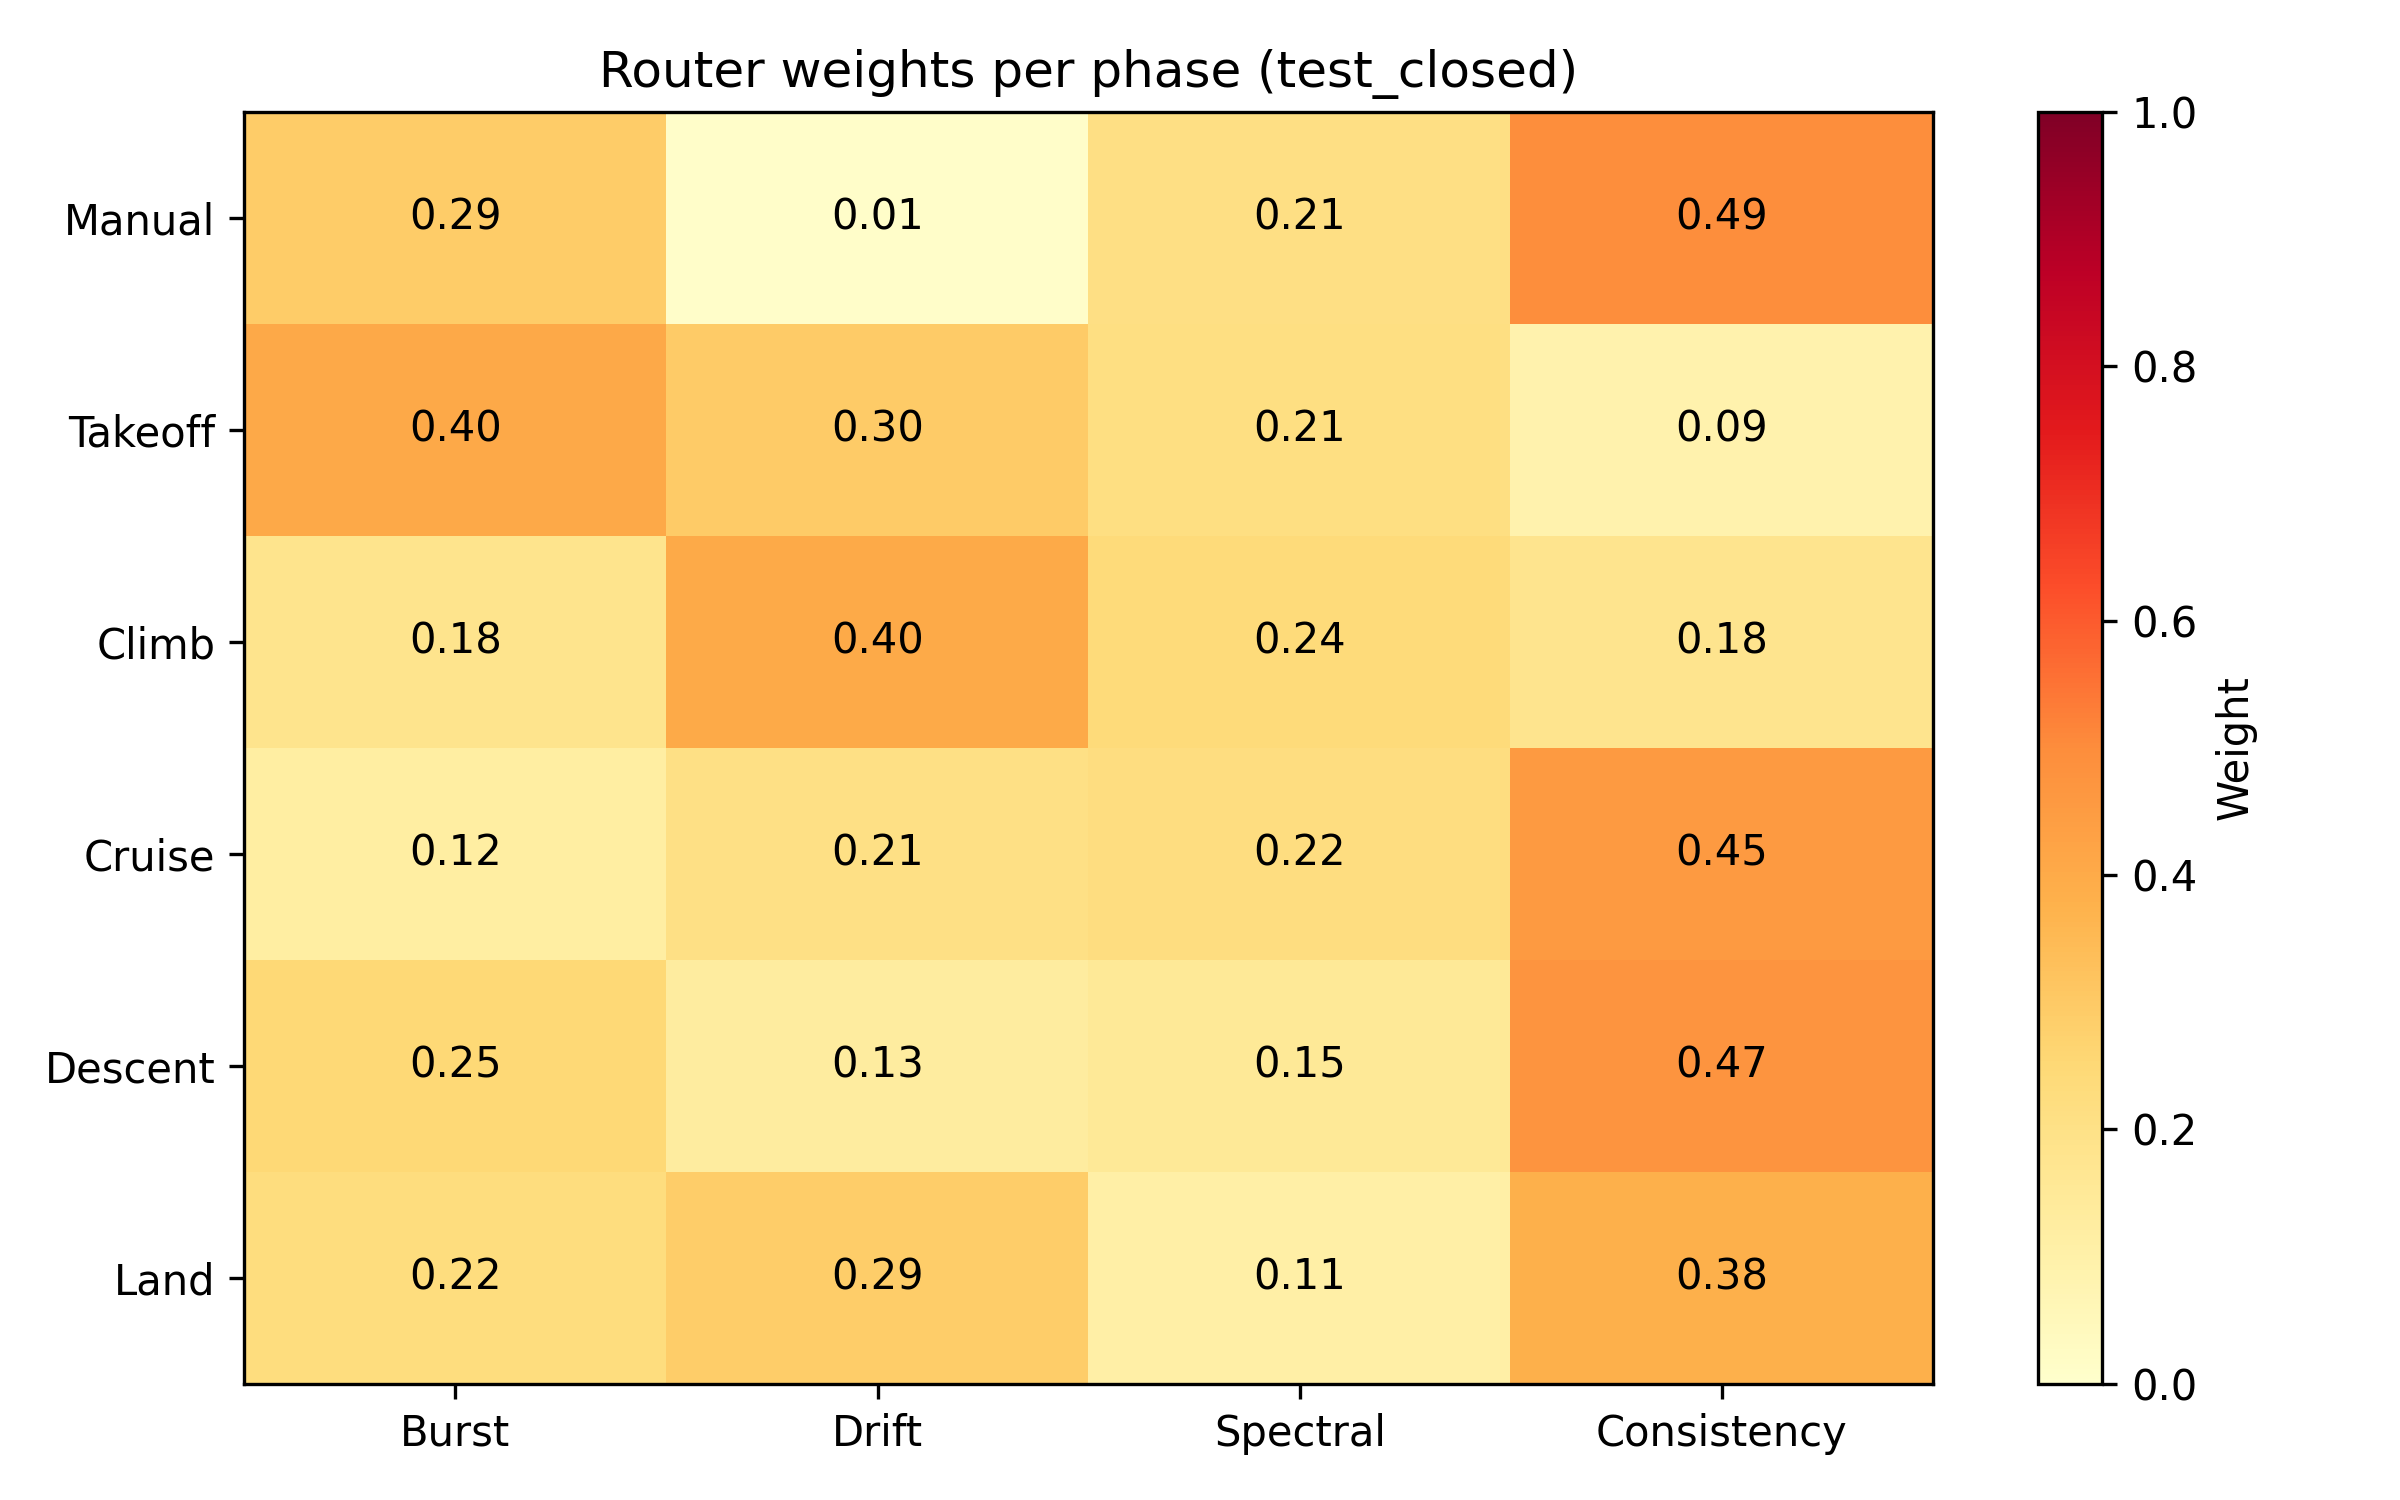
\includegraphics[width=0.95\columnwidth]{figures/router_heatmap_test_closed.png}
\caption{Routing weights per flight phase on test\_closed.}
\label{fig:router}
\end{figure}

\section{Conclusion}
FlightMoE v2 advances UAV anomaly detection by unifying phase-aware multimodal encoding and sparse expert routing. The key insight is that flight phase and fault mode jointly determine which features and experts are most informative. By learning sparse, phase-conditioned combinations of temporal, spectral, and consistency experts, the model achieves strong closed-set detection and substantially improved open-set generalization on RflyMAD. Future work will strengthen the physical-consistency GNN integration, explore online detection with streaming telemetry, and extend the framework to fault isolation.

\bibliographystyle{aaai}
\begin{thebibliography}{9}
\bibitem{rflymad} RflyMAD: A Dataset for Multicopter Fault Detection and Health Assessment.
\bibitem{shazeer2017} Shazeer et al. Outrageously Large Neural Networks: The Sparsely-Gated Mixture-of-Experts Layer. ICLR 2017.
\bibitem{gdn} Deng & Hooi. Graph Neural Network-Based Anomaly Detection in Multivariate Time Series. AAAI 2021.
\bibitem{madgan} Li et al. MAD-GAN: Multivariate Anomaly Detection for Time Series Data with Generative Adversarial Networks. ICANN 2019.
\bibitem{ganomaly} Akcay et al. GANomaly: Semi-Supervised Anomaly Detection via Adversarial Training. ACCV 2018.
\bibitem{hmm} Rabiner. A Tutorial on Hidden Markov Models and Selected Applications in Speech Recognition. Proceedings of the IEEE, 1989.
\end{thebibliography}

\end{document}
